\subsection{ A large-scale dynamical model}

Recently Chaudhuri et al. developed a large-scale dynamical model of the macaque neocortex \cite{chaudhuri2015large-scale}.
The model is based on recently acquired connectivity from tract tracing experiment \cite{markov2012weighted, markov2014anatomy}. Previously Markov et al. and Ercsey-Ravasz et al. 
The connectivity is strength is characterized by the fraction of labeled neurons (FLN); the FLN from area B to A is defined as:
\begin{equation}
FLN_{B\rightarrow A} = \frac{number\ of\ neurons\ projecting\ from\ B\ to\ A}{total\ number\ of\ neurons\ projecting\ to\ A}.
\end{equation}
The counting of the projecting neurons is done using retrograde tracer injections. For further details on the data acquisition see refs. \cite{markov2012weighted, markov2014anatomy, markov2011weight, kennedy2013data}. 
Not all FLN values between all brain areas of the macaque neocortex are know; therefore only a subnetwork of 29 areas, of which all FLN values are known, is used.
In addition to the FLN values, the fraction of supragranular layer neurons (SLN) is know of all connections between the areas. The SLN from area B to A is defined as
\begin{equation}
SLN_{B\rightarrow A} = \frac{number\ of\ supragranular\ neurons\ projecting\ from\ B\ to\ A}{number\ of\ neurons\ projecting\ from\ B\ to\ A}.
\end{equation}

Neurons mediating feedforward projections originate mostly from the supragranular layers.
Feedback projections, on the other hand, are primarily mediated by neurons originating from the infragranular layers of the cortex \cite{felleman1991distributed}. So if the connection from area A to B is mostly feedforward (feedback) $0.5 < SLN_{A\rightarrow B} < 1$ ($0 < SLN_{A\rightarrow B} <0.5$).
See appendix \ref{app:B} for information on cortical layers.
Using the SLN one can order the 29 brain areas such that the first area receives mostly feedback projections and its output is primarily feedforward, and the last area the other way around.
The hierarchical position can be quantified by assigning a number $h\in (0,1]$ each area \cite{chaudhuri2015large-scale, markov2014anatomy}.
The hierarchical position correlates to basal dentritic spine count. Spines are places were a other neuron can attach to. These  increase sharply from primary sensory areas to prefrontal areas.
Because this connections are primarily excitatory -- find ref -- the spine count is used as a proxy for excitatory connection strength, a gradient in the excitatory connection strength is introduced in the model \cite{elston2000pyramidal,elston2011pyramidal}.
Previously Chaudhuri et al. showed, using a simpler network architecture, that introducing a gradient in the connection strength leads to localized eigenvectors with a gradient in time constants \cite{chaudhuri2014diversity}.
To study the dynamics a threshold linear model was used, where each area is modeled as a single node which exists in an excitatory and an inhibitory version.
The resulting  network has 58 nodes. 
The time-evolution -- check -- of the firing rates of the nodes in the inhibitory and excitatory population, $\nu_I$ and $\nu_E$ respectively, are governed by the following equations,
\begin{equation}
\label{eq:wang_exc}
\tau_E \frac{d}{dt} \nu_E^i = - \nu_E^i + \beta_E \left[ \left( 1+\eta h_i \right) \left( w_{EE} \nu_E^i + \mu_{EE} \sum_{j=1}^N FLN_{ij} \nu_E^j \right) - w_{EI} \nu_I^i+ I_{ext,E}^i \right]_+
\end{equation}
\begin{equation}
\label{eq:wang_inh}
\tau_I \frac{d}{dt} \nu_I^i = - \nu_I^i + \beta_I \left[ \left( 1+\eta h_i \right) \left( w_{IE} \nu_E^i + \mu_{IE} \sum_{j=1}^N FLN_{ij} \nu_E^j \right) - w_{II} \nu_I^i+ I_{ext,I}^i \right]_+,
\end{equation}
with
\begin{equation*}
\left[x \right]_+ = \begin{cases}
	x, & \text{if } x>0\\
	0, & \text{if } x\leq0.
	\end{cases}
\end{equation*}
The parameter $\eta$ controls the effect of the gradient in the excitatory connection strength; $i$ and $j$ are the indices of the nodes; the hierarchical position of each node is $h_i$; $I_{ext,E}^i$ and $I_{ext,E}^i$ are the external inputs to node $i$ of the excitatory and inhibitory node, respectively.
All the other values of the parameters are taken from ref. \cite{binzegger2009topology}.

\begin{figure}[!ht]
\centering
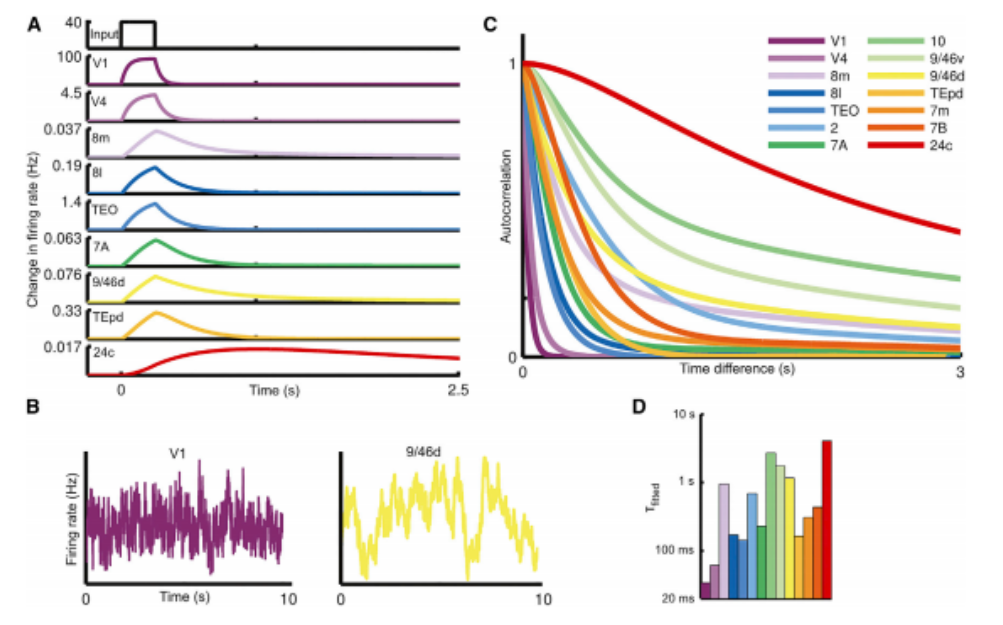
\includegraphics[scale=0.3]{wang_figures/mainfig}
\caption{A hierarchy of time scales in response to visual input.
(A) A pulse input to V1 in the primary visual cortex. Early areas can track the input with greater accuracy than latter areas, where the affect of the pulse persist for a longer period of time. The areas are ordered from earliest area, V1, in the hierarchy on top and the last area in the hierarchy, 25c, on the bottom.
(B) The response of areas V1 and 9/46d to white noise input to area V1.
(C) The autocorrelation of 14 areas decay over a wide range of time scales.
(D) The fitted time constants to the autocorrelations in (C). A trend is clearly visible: time constants increase along the hierarchy. Ordered from earliest area in the hierarchy, V1, on the left to the last area in the hierarchy, 25c, on the right.
Figure taken from \cite{chaudhuri2015large-scale}.
}
\label{fig:wang_fig}
\end{figure}

The response of the nodes in the network to pulsed input to area V1, in the primary visual cortex, is shown in figure \ref{fig:wang_fig} A. Early areas such as V1 and V4 can track the pulse with greater accuracy than latter areas; e.g., 24c where the response to the pulse is smeared out over several seconds.
As a measure for the time constant of each area the decay time of the autocorrelation of the response to white noise input to area V1 are used \ref{fig:wang_fig} B and C.
The decay time of the areas tend to increase along the hierarchy \ref{fig:wang_fig} D.
Though a trend is ... , the time scales do not increase monotonously along the hierarchy. 

\begin{figure}[!ht]
\centering
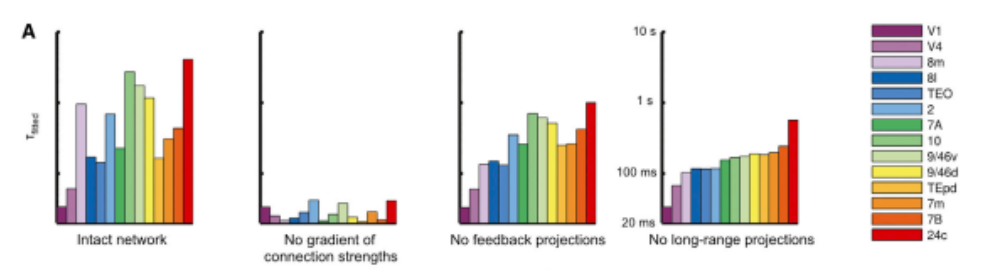
\includegraphics[scale=0.3]{wang_figures/time_consts}
\caption{The timescales for different models. Far left: the intact network. Second from the left: the model without the gradient in excitatory connection strength; i.e., $\eta=0$ in eqns. \ref{eq:wang_exc} and \ref{eq:wang_inh}. The trend in the time constants is destroyed, and all time constants are decreased significantly, mostly in area further in the hierarchy.
Third from the left: the time constants of the areas with the feedback projections removed. The decrease of the time constants in the areas higher up in the hierarchy shows the tendency of these areas to form feedback loops.
Far right: the network without long-range projections. In this network the time constants follow the same order as the hierarchy.
Figure taken from \cite{chaudhuri2015large-scale}.
}
\label{fig:wang_time_consts}
\end{figure}

In order to show that the gradient in the connection strength is indeed the origin of the gradient in the time scales  different aspects of the model are removed; see figure \ref{fig:wang_time_consts}.
Removing the hierarchy in excitatory connection strength destroys the trend in the time scales; there is no longer a a relation ship between the position in the hierarchy and the time scale of the area.
This is a result from  the decrease in time scales of areas further along the hierarchy.
Removing the feedback projections, determined by the SLN value \cite{felleman1991distributed}, from the connectivity matrix results in a decrease in the range of the time scales, showing that slow areas tend to form excitatory loops.
Without long-range projections, e.i. setting all $FLN_{ij}=0$ for all $i$ and $j$, the order of the areas is the same when the areas are ordered by time constant or hierarchical position.

\begin{figure}[!ht]
\centering
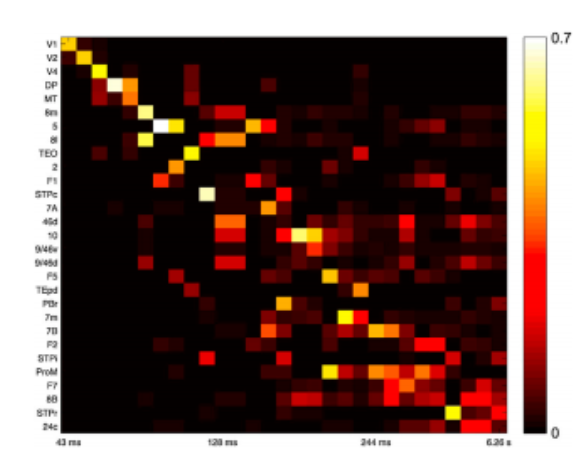
\includegraphics[scale=0.4]{wang_figures/eigenvecs}
\caption{ The eigenvectors of the linearized equations. The eigenvectors are represented by the columns. The area corresponding to the entry of the eigenvector are shown on the left, ordered by hierarchical position with the first area on top.
Figure taken from \cite{chaudhuri2015large-scale}.
}
\label{fig:wang_eigenvecs}
\end{figure}

Neglecting the non-linearity in the model, replacing $[x]_+$ by  $[x]=x$ in eqns. \ref{eq:wang_exc} and \ref{eq:wang_inh}, one can use linear system analysis. In a linear system the activity is the weighted sum of the eigenvectors \cite{rugh1993linear}. The timescales of the eigenvector are given by $\tau = 1/Re\{\lambda\}$. The eigenvectors of the linearized model are localized, in the sense that each eigenvector has a significant amplitude in only a small number of entries \ref{fig:wang_eigenvecs}. The eigenvectors that are localized in the areas early in the hierarchy have a short time scale ($~43 ms$), and the last areas in the hierarchy have a timescale that is larger by several orders of magnitude ($~6 s$). This corroborates the findings in figure \ref{fig:wang_fig}: areas early in the hierarchy have a short time scale and areas further up in the hierarchy have an increasingly longer timescale.

